\section{Design}

\subsection{High Level Overview}

The system will comprise 3 parts required to simulate and program a proprietary processor. It will include a virtual machine to emulate the execution of binary machine code catridges, an assembler to translate higher level assembly code into machine code, and finally a compiler for a higher level language to easily program complex applications to run on the processor.

The virtual machine consists of two main processes, the debugger and interpreter. The interpreter will continiously step through memory, decoding and executing instructions sequentially whilst displaying the contents of VRAM through the pixel display.

\shadowbox{
    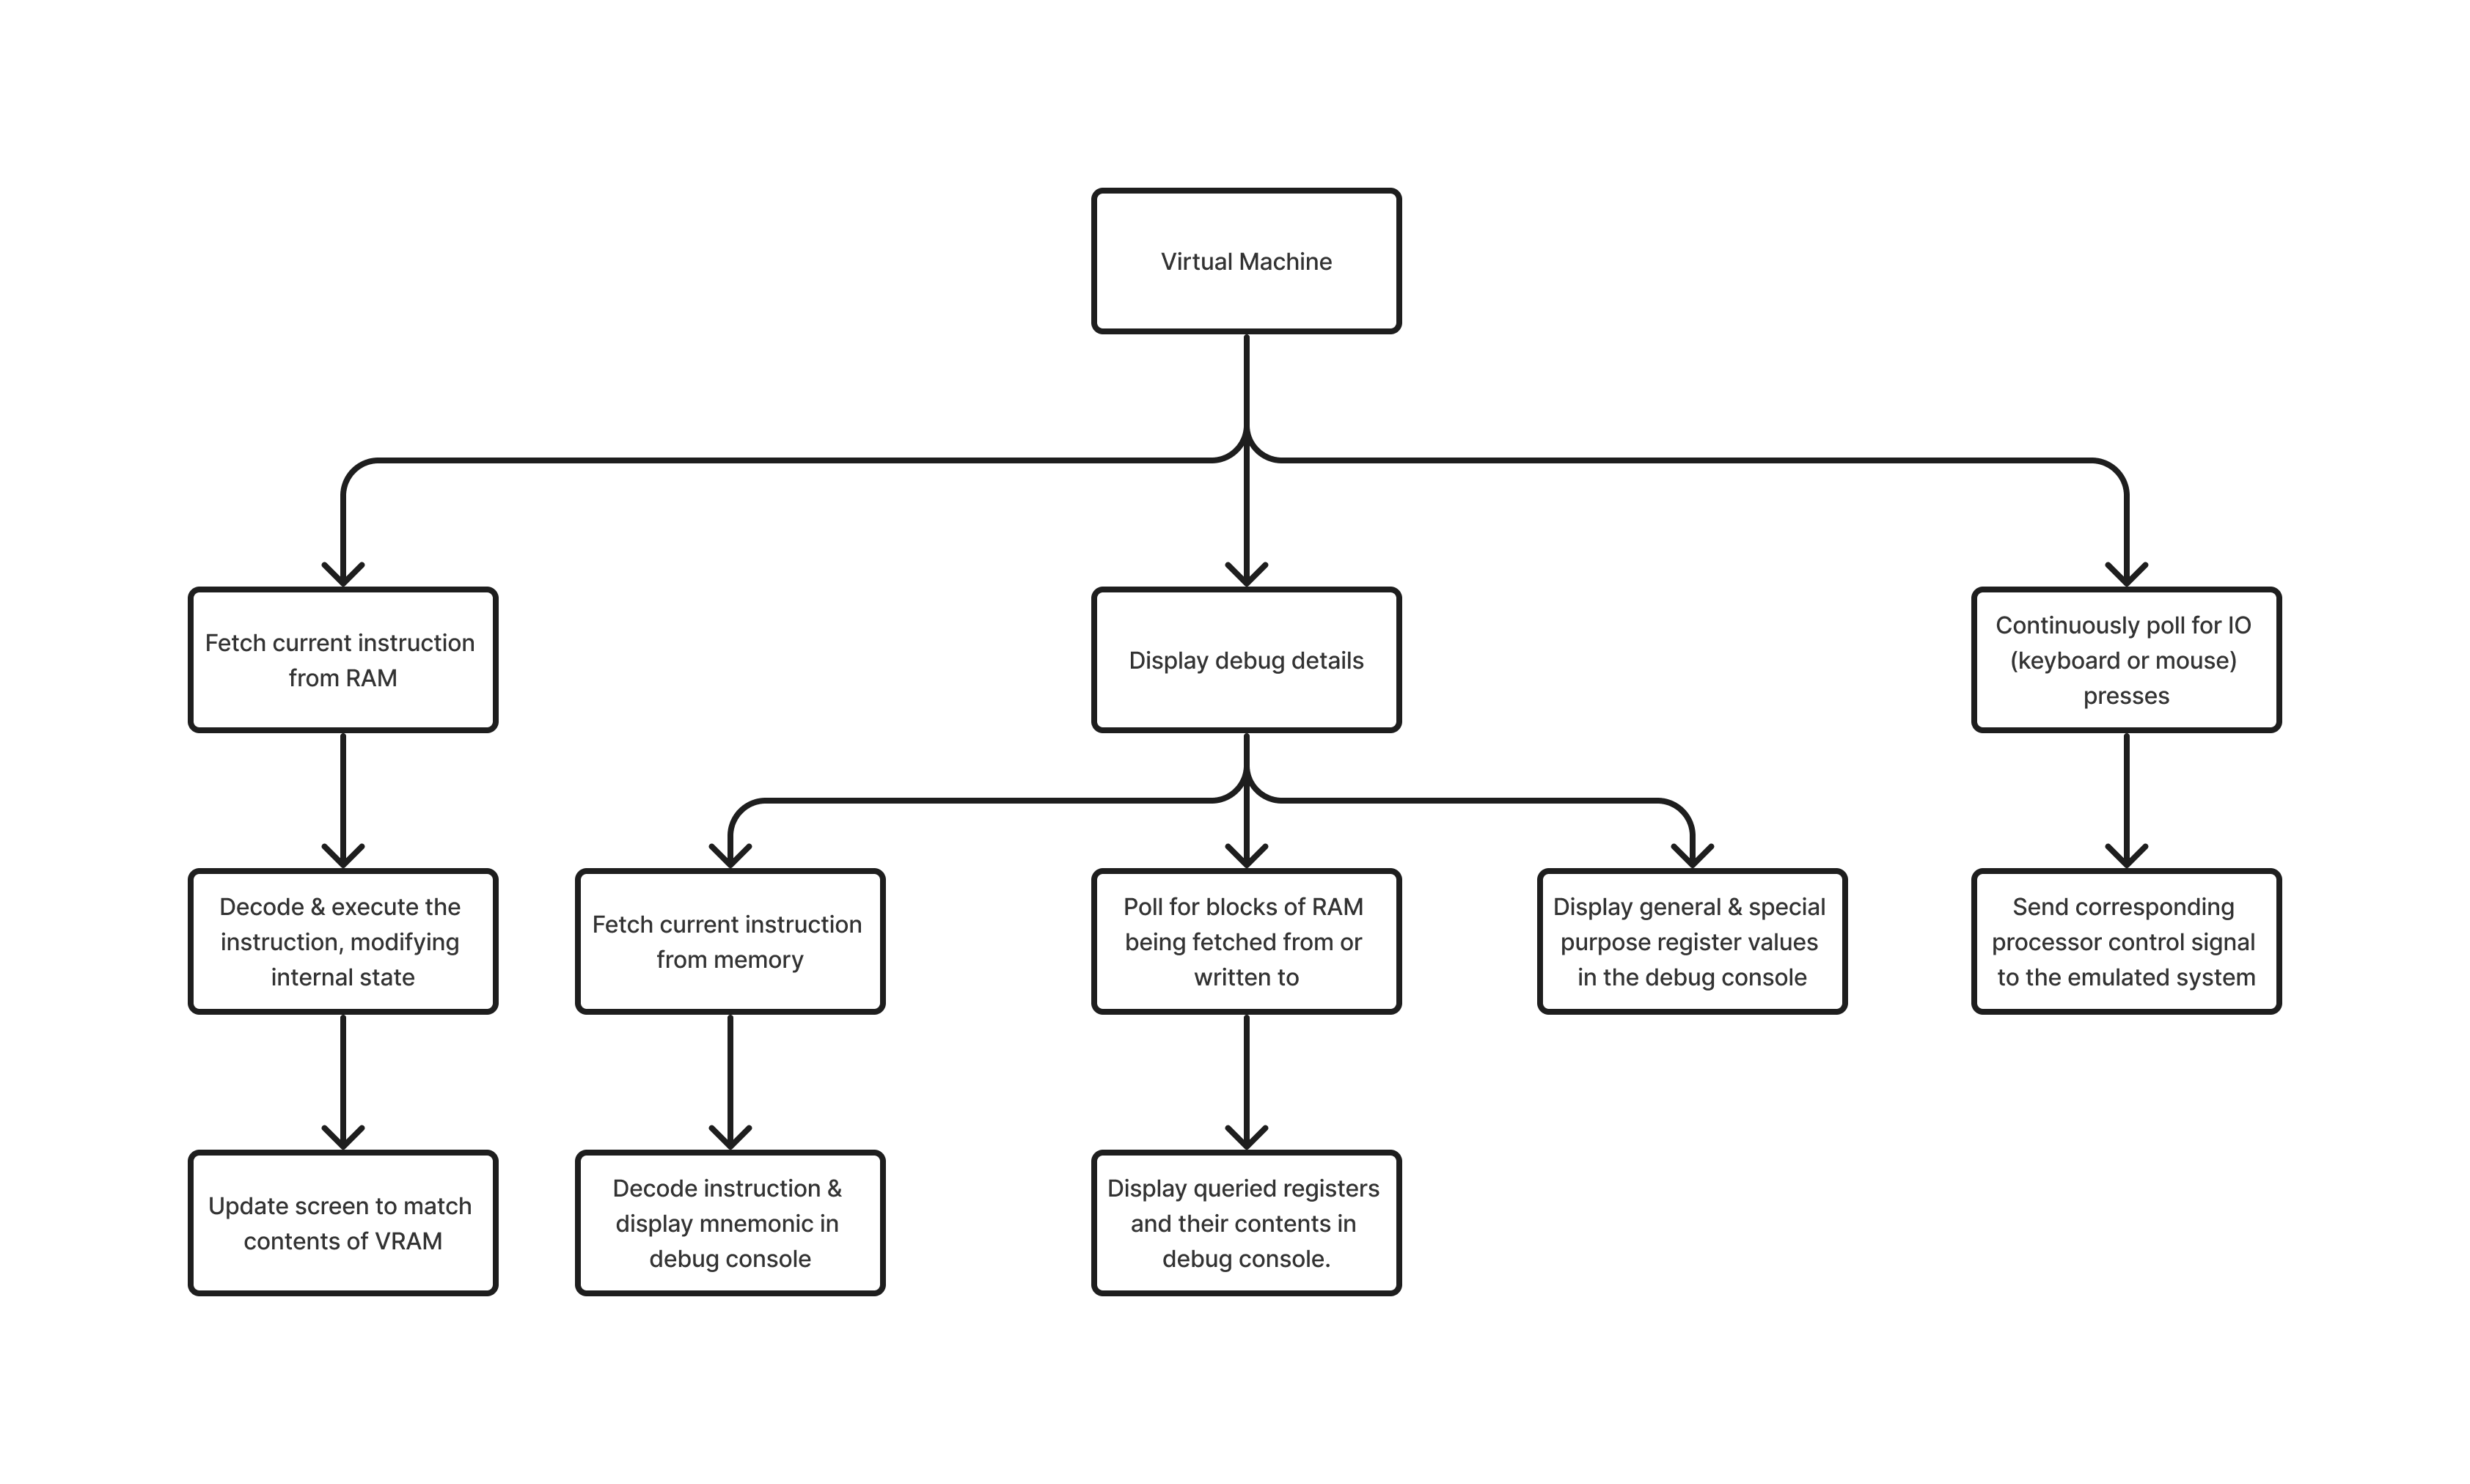
\includegraphics[width=14cm]{Virtual Machine Flowchart.png}
}

\bigskip

The assembler consists of a single pipeline for transforming ASCII assembly programs into binary machine code. The files are loaded into the interpreter which stores their contents in a string. The contents are tokenised and parsed into a sequence of assembly language instructions. These instructions are translated into binary machine code according to the instruction set architecture (defined in \ref{sec:ISADesign}).

\bigskip

\shadowbox{
    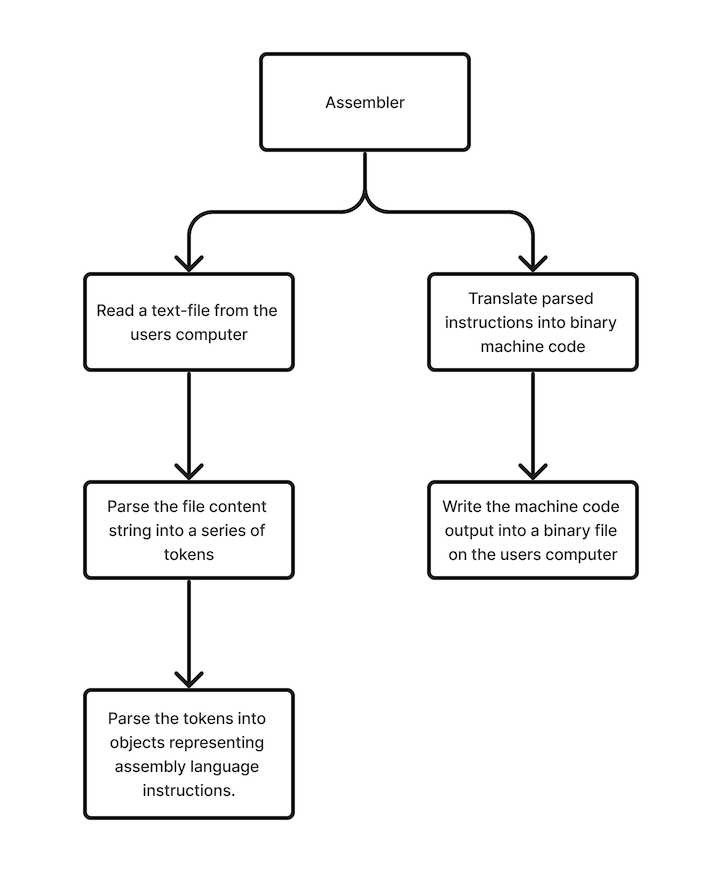
\includegraphics[width=7cm]{Screenshot 2024-06-24 at 19.15.56.png}
}

\bigskip

Much like the assembler, the compiler takes an ASCII program, converts it into tokens and parses it into an Abstract Syntax Tree (AST) representing the structure and order of operations of the program. This AST is converted into an internal representation (IR) designed to help easily locate potential optimisations in the source code (e.g. pre-calculating arithmetic or removing redundant code), these optimisations are made and the IR is converted into an intermediate assembly language due to the presence of high level optimisations such as labels and macro-instructions. Finally, this assembly code is inserted into the assembler and the produced machine code is stored as a file on the users computer. 

\bigskip

\shadowbox{
    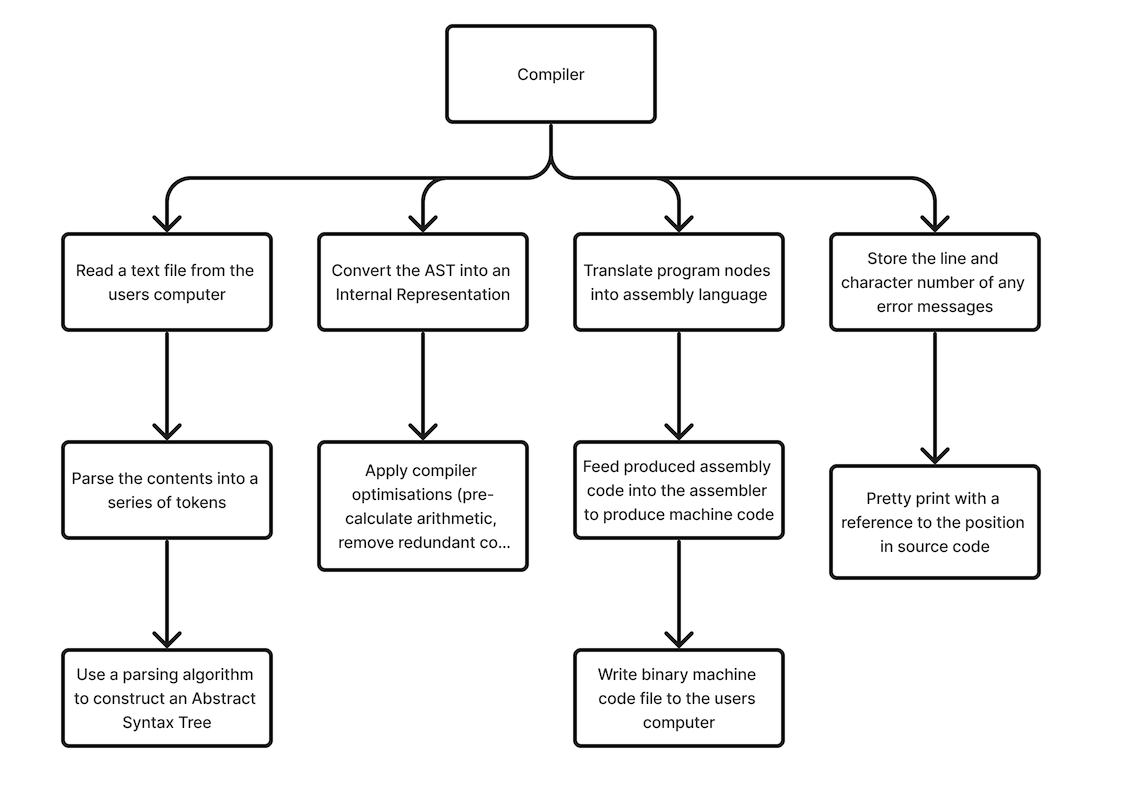
\includegraphics[width=10cm]{Screenshot 2024-06-24 at 19.30.50.png}
}

\subsection{Component Design}
\subsubsection{Instruction Set Architecture}

\subsubsubsection{Computer Architecture}
Registers, Status, PC, MAR.....

\subsubsubsection{Arithmetic and Logic Unit}
\label{sec:ISADesign}
The core of any instruction set is the Arithmetic Logic Unit (ALU) so I began by designing an interface for that. I decided on 2 16-bit inputs to the ALU, which for the purpose of my architecture will only take register values. There are 6 ALU control bits that enable further operations aside from the NOT, AND, and ADD with their own dedicated logic circuits. Below is the chip interface diagram for the ALU I will use in this processor.

\bigskip

\shadowbox{
    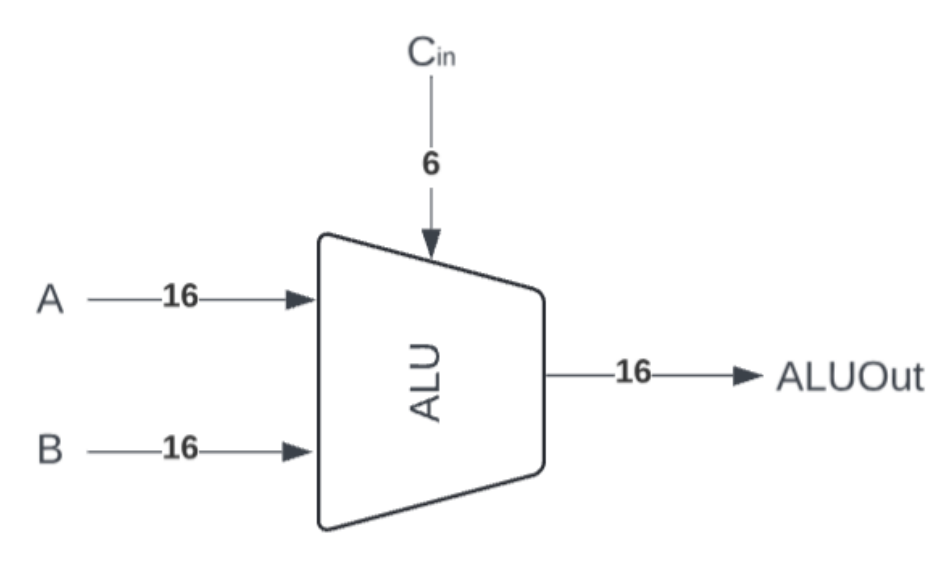
\includegraphics[width=6cm]{Screenshot 2024-07-20 at 19.36.41.png}
}

\bigskip

Different configurations of these 6 ALU control bits can produce different arithmetic and logical operations, detailed in the table below:

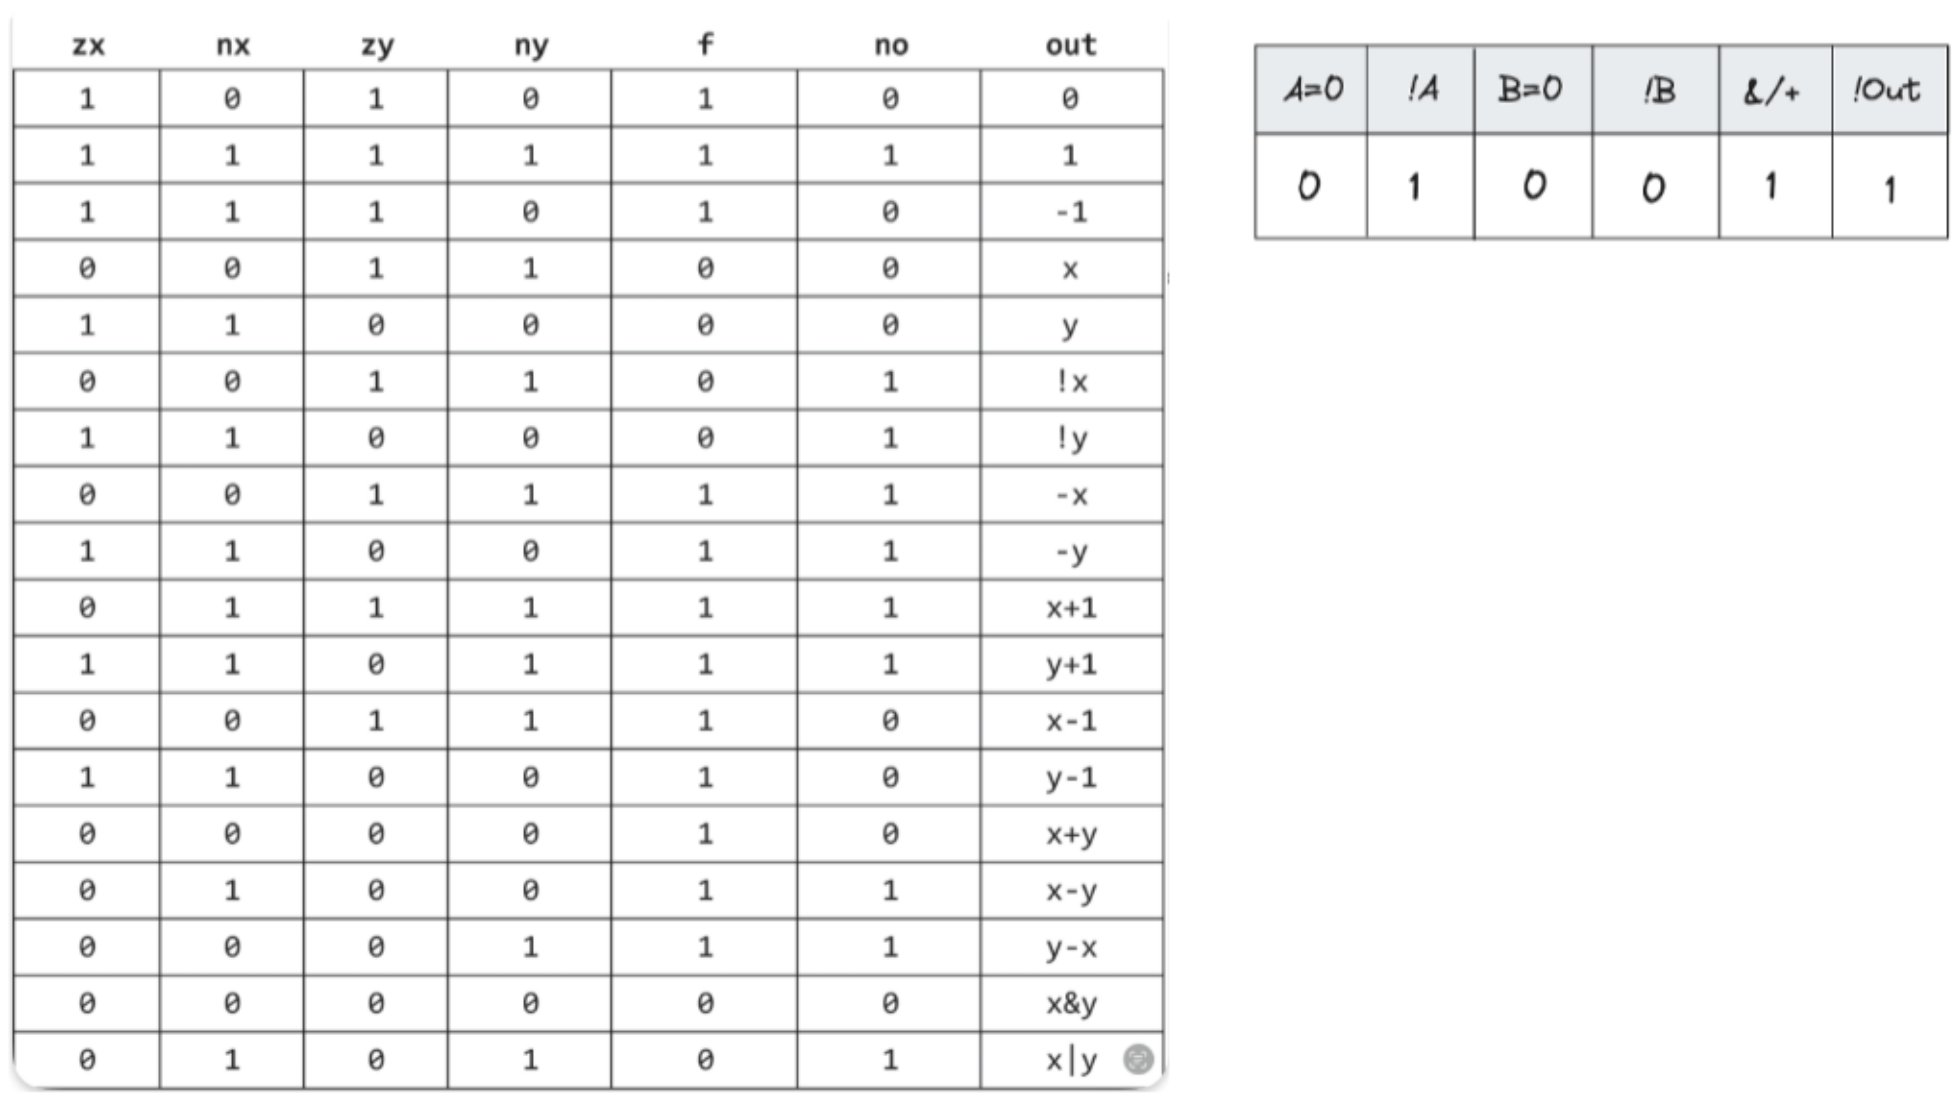
\includegraphics[width=11cm]{Screenshot 2024-07-20 at 19.37.03.png}
% 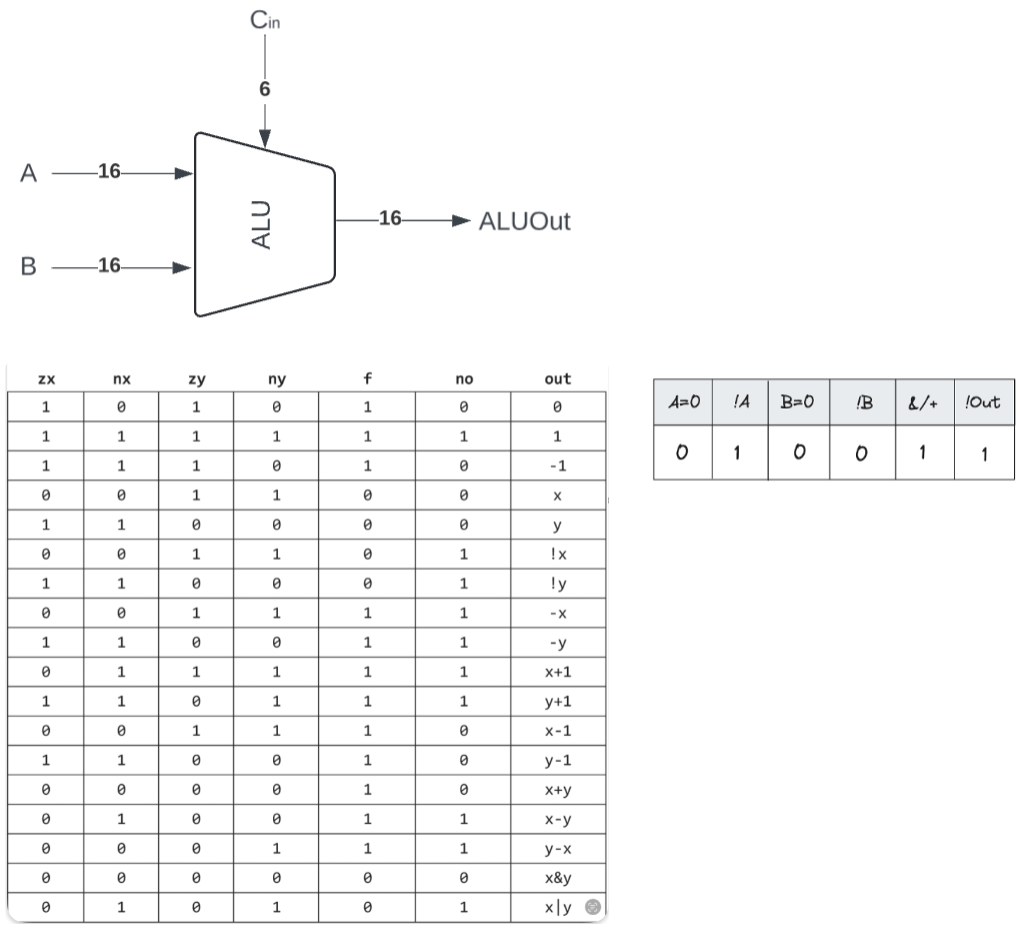
\includegraphics[width=12cm]{Screenshot 2024-07-12 at 16.47.22.png}

% \bigskip

\subsubsubsection{Assembly Language}

I decided to use a MIPS instruction set architecture, minimising the number of instructions supported by the processor. I settled on 3 instruction types: R-type instructions (performing ALU operations on register values), I-type instructions (load and store data between registers and memory), and J-type instructions (conditional jumps to different points in memory). From these 3 types, the following instruction set can be constructed, demonstrated with a program to multiple two numbers stored in memory. (\texttt{'[]'} are used to indicate a memory address):

\begin{lstlisting}[language=C]
LI-type: li
I-type: sw, lw
R-type: add, sub, and, or, not
J-type: jmp, jlt, jle, jeq, jge, jgt, jal

// multiply the numbers in memory address 0xb000 and 0xb001, and write the answer to 0xb002
li r0, 0xb000
lw r1, [r0]

li r0, 0xb001
lw r2, [r0]

.loop
    // if r2 is 0, break
    li r0, 0

    li r31, [.store]
    jle r2, r0, [r31]

    add r1, r1, r1

    li r0, 1
    sub r2, r2, r0

    li r0, [.loop]
    jmp [r0]

.store
    li r0, [0xb002]
    sw r1, [r0]
\end{lstlisting}

\subsubsubsection{Machine Code Encoding}

Below is the breakdown of how R/I/J type instructions are represented in binary, broken down into their respective fields. All instructions have a 2-bit opcode which dictates the type of instruction (and consequentially which of 4 encoding types should be used when decoding the instruction). 

\begin{itemize}
    \item \texttt{00}: LI-type instructions \textit{(to load immediate values into registers)}
        \begin{itemize}
            \item \texttt{5-bits rd}: the register in which to store the immediate value.
            \item \texttt{16-bits im}: a 16-bit signed integer.
        \end{itemize}
    \item \texttt{01}: I-type instructions \textit{(to transfer data between CPU registers and RAM)}
        \begin{itemize}
            \item \texttt{1-bit lw/sw}: determines whether to load from or write to RAM.
            \item \texttt{5-bits rd}: the register to store the word loaded from memory, or containing the data to be written.
            \item \texttt{5-bits rs}: the register containing the address of the location in memory to be read from or written to.
        \end{itemize}
    \item \texttt{10}: R-type instructions \textit{(to perform operations between two registers)}
        \begin{itemize}
            \item \texttt{6-bits Cin}: the control bits determining the operation to be carried out on the registers in the ALU.
            \item \texttt{5-bits rd}: the register in which to store the result of ALU operations.
            \item \texttt{5-bits rs}: the first of two input registers to the ALU.
            \item \texttt{5-bits rt}: the second of two input registers to the ALU.
        \end{itemize}
    \item \texttt{11}: J-type instructions \textit{(to conditionally jump to another instruction in memory)}
        \begin{itemize}
            \item \texttt{3-bits <=>}: control bits to determine the jump condition.
            \item \texttt{1-bit al}: determines whether to store the return address in rd.
            \item \texttt{5-bits rd}: the register to contain the return address of the jump.
            \item \texttt{5-bits rt}: the register containing the memory address to jump to.
        \end{itemize}
\end{itemize}
 
\bigskip

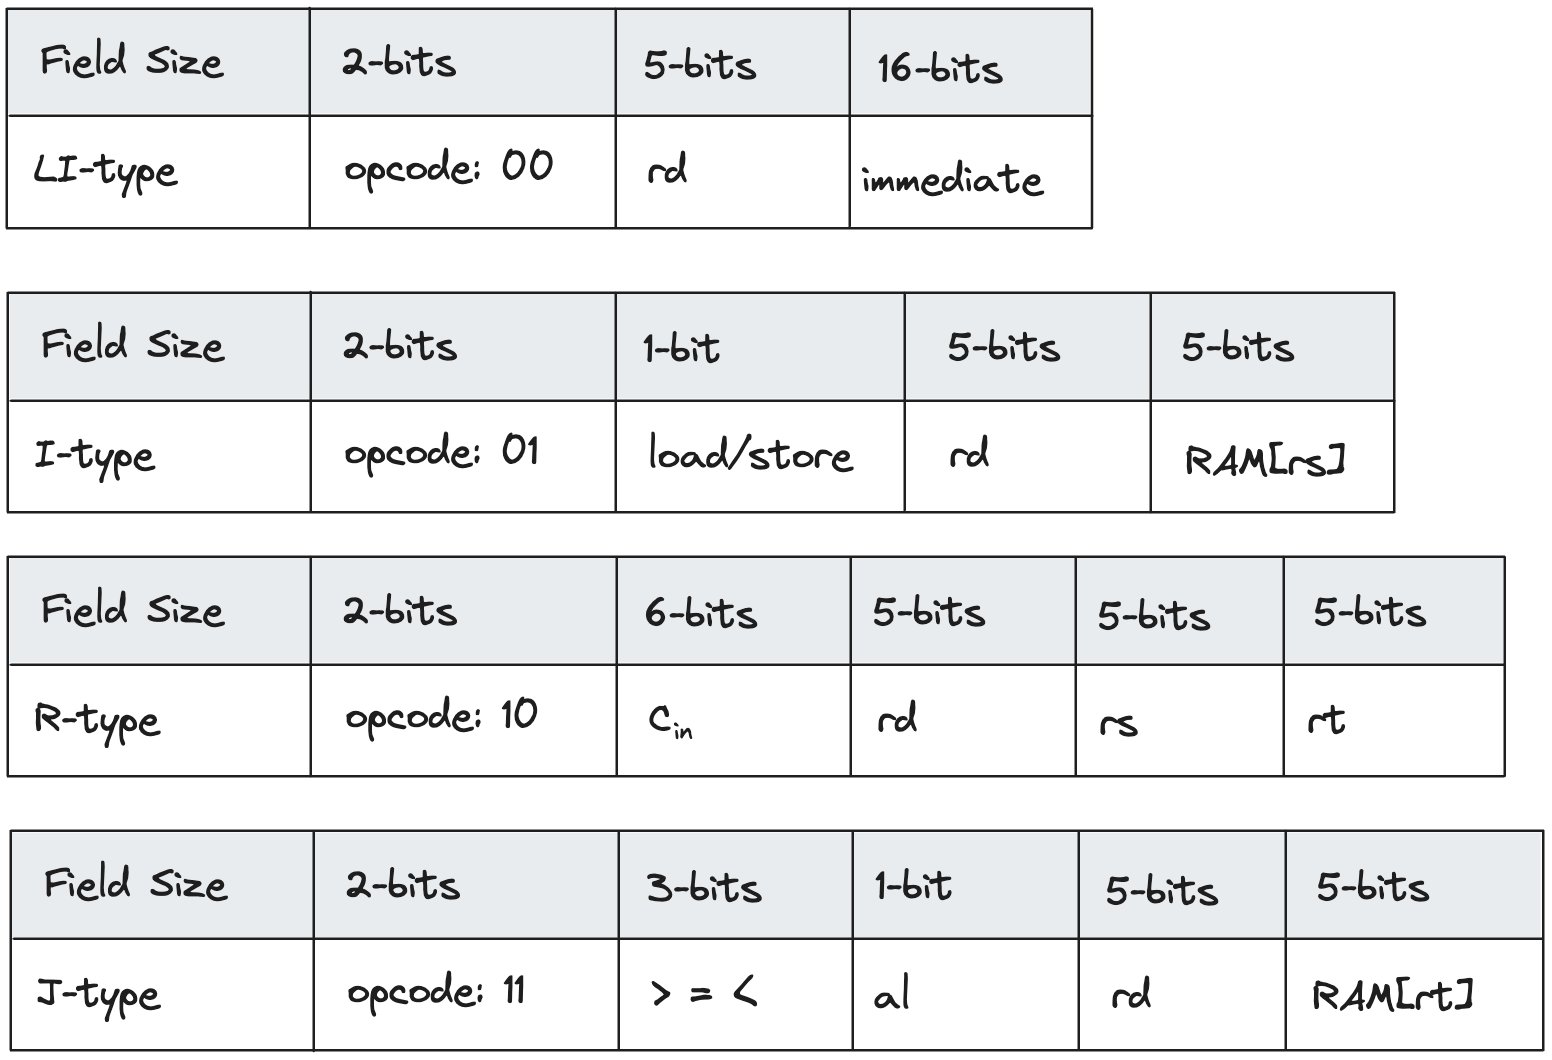
\includegraphics[width=12cm]{Screenshot 2024-07-21 at 17.47.26.png}

\bigskip

Below is a simple program to demonstrate the process of encoding between assembly language and machine code following the specification above.

\begin{lstlisting}
li r5, 14        // 00 00101 00000000 00001110

li r30, 0xb000   // 00 11110 10110000 00000000
lw r4, [r30]     // 01 0 00100 1110

li r30, [0x010a] // 00 11110 00000001 00001010

// a cmp is a sub without storing the result
cmp r5, r4       // 10 010011 00000 00101 00100
jge [r30]        // 11 110 0 00000 11110
\end{lstlisting}

\subsection{Virtual Machine}
\subsubsection{Data Structures}
\subsubsection{Algorithms}